%% ==============================
\chapter{\iflanguage{ngerman}{Ergebnisse}{Results}}
\label{sec:results}
%% ==============================
\section{Hardware }

\subsection{Robot Platforms}
RSI used for communication with the robots
\subsubsection{KUKA KR 16-2}

\missingfigure{Please add some figures}

\subsubsection{KUKA KR 5}
\missingfigure{Please add some figures}



\subsection{Network}


\subsection{Computer}




\section{The Setup Used for Evaluation}
Different middlewares:
\begin{enumerate}
    \item Eclipse Cyclone DDS
    \item eProsima Fast DDS
    \item Zenoh
\end{enumerate}
Different Publishing types
\begin{enumerate}
    \item Node topology
    \item Publish trigger
    \item Publish type 
\end{enumerate}
\todoin{should probably test with different network workloads...}

\begin{table}[]
\begin{tabular}{cl|lll}
\multicolumn{1}{l}{}                                  &                                                          & \multicolumn{3}{c}{Middleware}                                                                                \\ \cline{3-5} 
\multicolumn{1}{l}{}                                  &                                                          & \multicolumn{1}{c|}{Eclipse Cyclone DDS} & \multicolumn{1}{c|}{eProsima Fast DDS} & \multicolumn{1}{c}{Zenoh} \\ \hline
\multicolumn{1}{c|}{\multirow{2}{*}{Node topology}}   & \multicolumn{1}{c|}{One node per sub-controller manager} & \multicolumn{1}{l|}{}                    & \multicolumn{1}{l|}{}                  & \multicolumn{1}{l|}{}     \\ \cline{2-5} 
\multicolumn{1}{c|}{}                                 & One node per interface                                   & \multicolumn{1}{l|}{}                    & \multicolumn{1}{l|}{}                  & \multicolumn{1}{l|}{}     \\ \hline
\multicolumn{1}{c|}{\multirow{2}{*}{Publish trigger}} & Publish on timer                                         & \multicolumn{1}{l|}{}                    & \multicolumn{1}{l|}{}                  & \multicolumn{1}{l|}{}     \\ \cline{2-5} 
\multicolumn{1}{c|}{}                                 & Publish on value change                                  & \multicolumn{1}{l|}{}                    & \multicolumn{1}{l|}{}                  & \multicolumn{1}{l|}{}     \\ \hline
\multicolumn{1}{c|}{\multirow{2}{*}{Publish type}} & Normal publisher                                         & \multicolumn{1}{l|}{}                    & \multicolumn{1}{l|}{}                  & \multicolumn{1}{l|}{}     \\ \cline{2-5} 
\multicolumn{1}{c|}{}                                 & Real-time publisher                                      & \multicolumn{1}{l|}{}                    & \multicolumn{1}{l|}{}                  & \multicolumn{1}{l|}{}     \\ \hline
\end{tabular}
\end{table}

\section{test 1}
\begin{figure}[htbp]
	\centering
	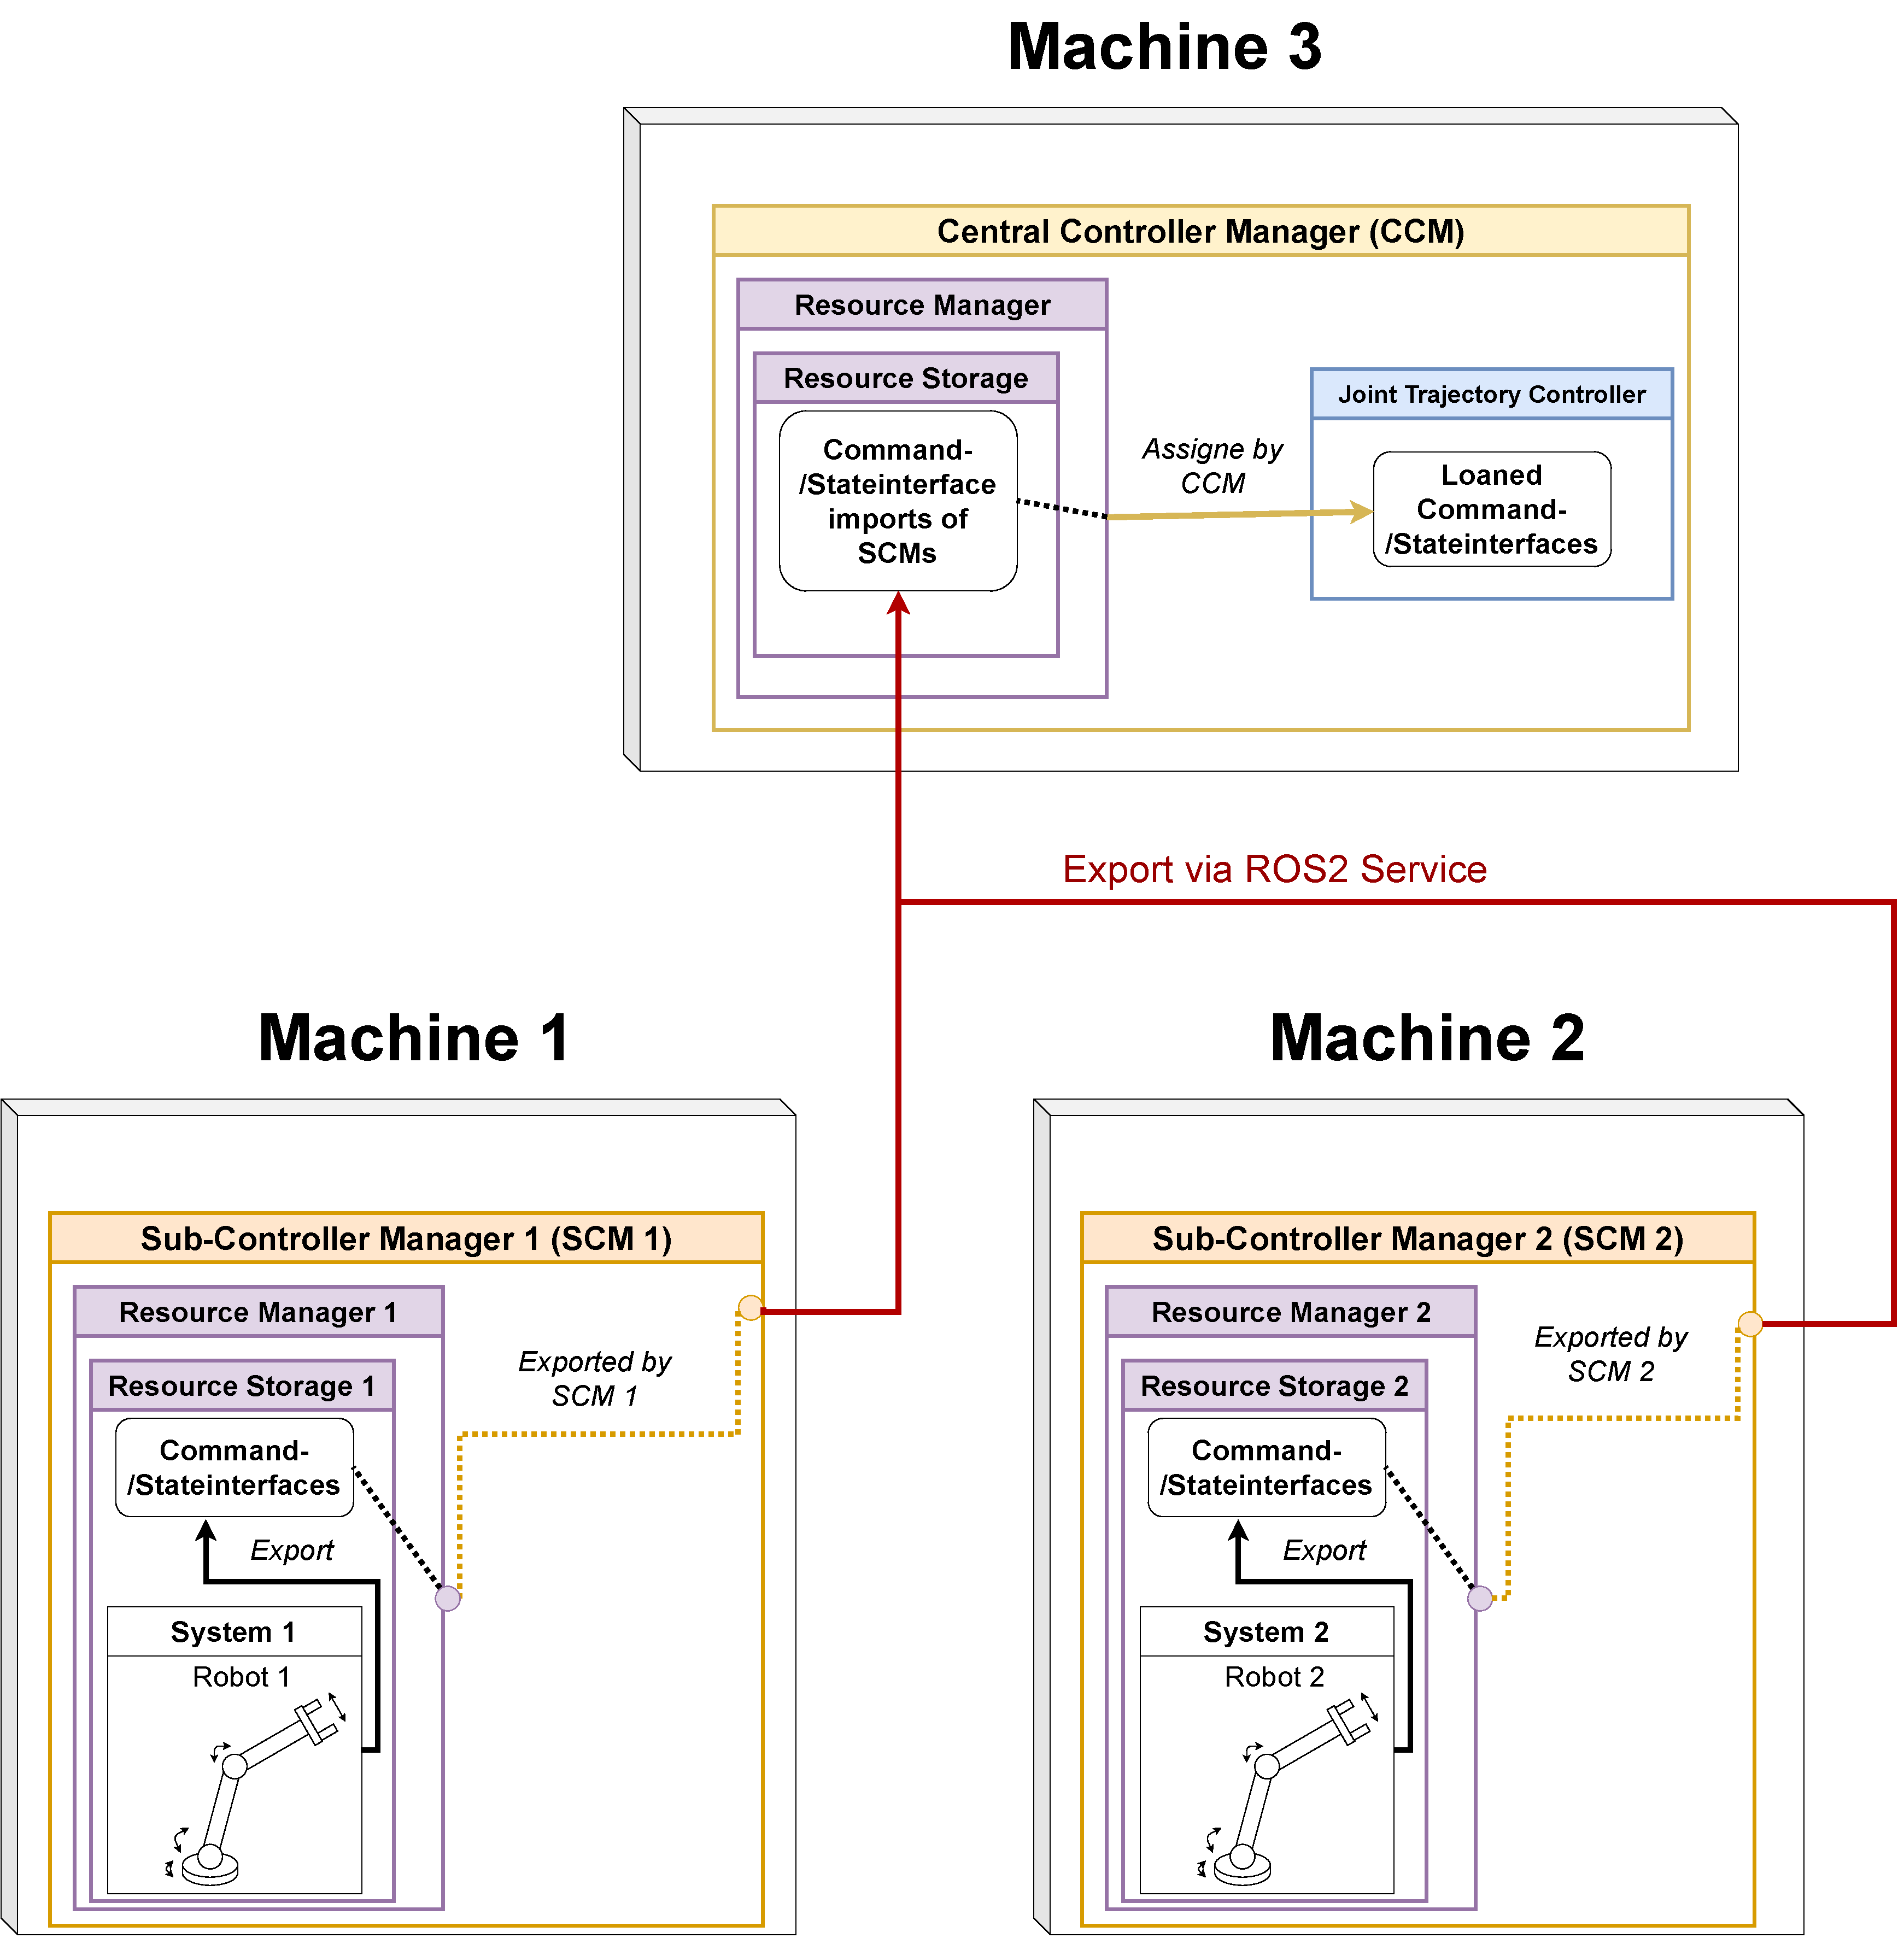
\includegraphics[width=1\textwidth]{Figures/c6/test_scenario_1.drawio.pdf}
	\caption{Schematic overview of the conceptual design of the system for the first test.}
	\label{c6_fig_test_scenario_1}
\end{figure}
\begin{figure}[htbp]
	\centering
	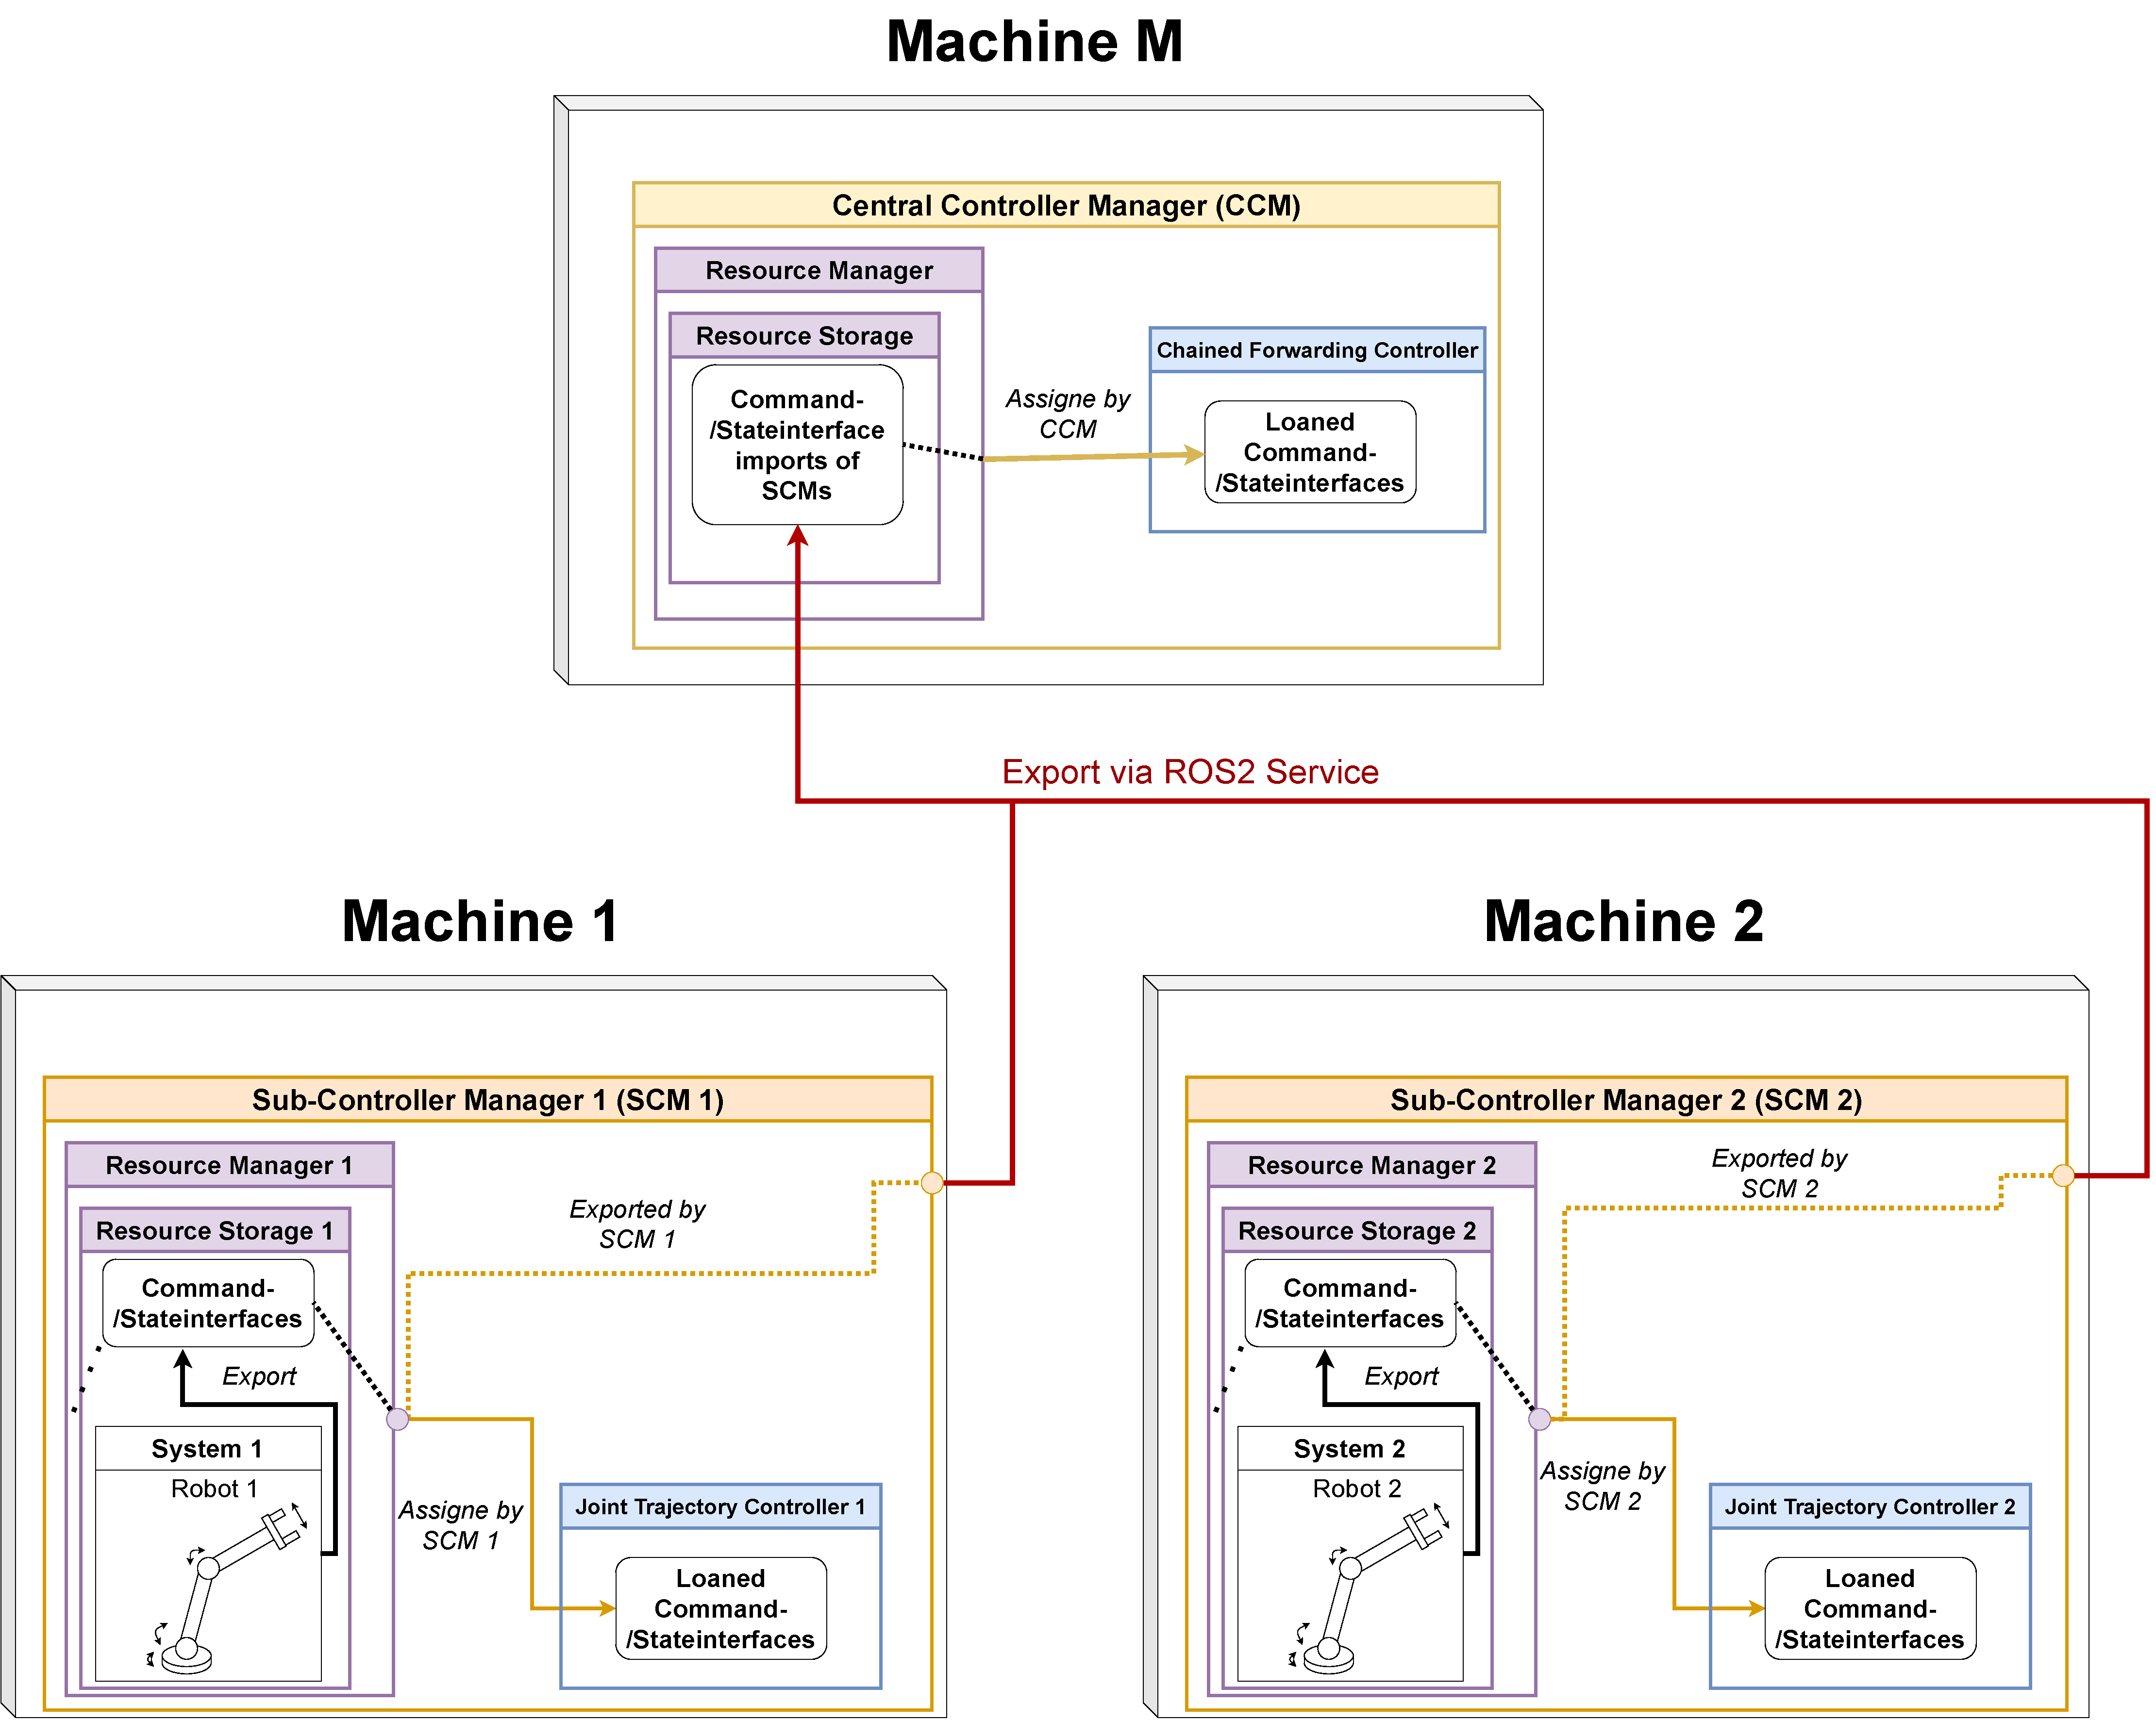
\includegraphics[width=1\textwidth]{Figures/c6/test_scenario_2.drawio.pdf}
	\caption{Schematic overview of the conceptual design of the system for the second test.}
	\label{c6_fig_test_scenario_2}
\end{figure}

